%========================================
%                            Chapter                            
%======================================== 
\chapter{Introduction}

%	With the rapid development of technology, smartphones nowadays can provide services including, but not limited to, email checking, web browsing, online shopping, game playing, music listening, video shooting, and GPS navigation. S
%	
%	As a results, billions of people use smartphones in their daily lives. The security and privacy on smartphones ha
%	
%	
%Almost everyone has a smartphone. They all suffer from security and privacy problems, such as authentication and privacy leakage. Existing solutions including .... We utilize the embeded sensors on smartphone. In detail, ....

%========================================
%                            Section                             
%======================================== 	 
\section{Security and Privacy on Smartphones}
Compared to traditional feature phones which are capable of voice calls and text messages,
%
smartphones bring many more applications including, but not limited to, email checking, web browsing, online shopping, game playing, music listening, video shooting, and GPS navigation.
%
%enable users to check their email, browse the web, post updates to social media sites, shop online, play games, listen to music,  shoot photos, and so on.
%
%can provide users with many more services such as email checking, web browsing, game playing, music listening, social chatting, video shooting, and so on. 
%
%
With such extensive capabilities, smartphones have become ubiquitous and all-pervasive.
%
Indeed, the total number of smartphone users worldwide is over 3 billion this year -- nearly 40\% of the human population, according to reports issued by several market-research firms~\cite{report2018newzoo,report2019forrester}. 


The increasing of smartphone users also increases the importance of protecting the security and privacy on smartphones. 
%
Smartphones hold our important personal information such as photos and videos, SMS, email, contact list, social media accounts, etc. But existing powerful OSs and applications are not enough to protect those infromation~\cite{ali2019security}. For example, Google confirms an Android camera security threat where `hundreds of millions' of users are affected~\footnote{\url{https://www.forbes.com/sites/daveywinder/2019/11/19/\\google-confirms-android-camera-security-threat-hundreds-of-millions-of-users-affected}}. The attackers can control the Google Camera app to take photos and/or record videos through a rogue application~\footnote{\url{https://www.checkmarx.com/blog/how-attackers-could-hijack-your-android-camera}} that has no permissions to do so. 


Researches have done extensive study on the security and privacy problems about smartphones~\cite{ali2019security,zaidi2016survey,chin2012measuring,khan2015survey}. They have classified the smartphone problems into four categories~\cite{zaidi2016survey}:

\begin{itemize}
	\item Authentication. There are mainly three ways to authenticate humans: something you know (PIN, graphical pattern, password, etc.), something you have (One-time passcode (OTP) via SMS, offline OTP using apps, paired devices, etc.), and something you are (voice, face, fingerprint, etc.). However, every method has pros  and cons and no one is perfect. Researchers keep proposing new methods as surveyed in~\cite{teh2016survey,spolaor2016biometric,mahfouz2017survey,vongsingthong2015survey,gupta2018demystifying}.  In this thesis, we also propose a new authentication system {\uu}. We also improve the existing voice authentication system against spoofing attacks in {\mv}.
	
	\item  Data Protection and Privacy. Smartphones, like computers, bring the same concerns: whether or how data is shared with third parties. Researchers have studied data protection and privacy problems from different perspective~\cite{muslukhov2012understanding,boyles2012privacy,wang2015know}. Existing solutions are mainly designing protocols~\cite{zegers2015lightweight,urien2013framework} or utilizing cryptography~\cite{patel2016integrated,han2016enhancing}.
	
	\item Vulnerabilities. Smartphone vulnerabilities include the following: system faults/defects, insufficient management of applications, insecure wireless networks, and lack of user awareness. The hardware and operating systems on smartphones are evolving and upgrading all the time. They are inevitable to have defects at a certain stage. Developers are publishing new applications every day. Detecting malware, hacking, and other harmful codes embedded in the apps is still an open problem~\cite{idrees2017pindroid}. Even when the smartphone is secure, its connection to an insecure network can still cause S\&P problems. Moreover, user awareness is another critical factor for smartphone security. A previous research~\cite{van2013modifying} suggests that 35\% of smartphone users do not lock their devices to prevent unauthorized persons from using them. Improving the user awareness level is urgent~\cite{koyuncu2019security}.
	
	\item Attacks. Researchers have studied various attacks on smartphones. For example, researchers propose theft detection algorithms to protect smartphones against physical attacks~\cite{chang2016smartdog}, and propose liveness detection algorithms to prevent replay attacks~\cite{zhang2016voicelive}.  However, there are many other attacks unrevealed or uninvestigated.  In this thesis, we propose the {\attackName} attack, which turns smartphones into spy bugs. 
\end{itemize}




\section{Smartphone Sensors: Causes  or Solutions}
There are no universally applicable solutions to solve the aforementioned security and privacy issues, so we conduct our research in a case study manner. We propose {\spp} to show how smartphones get eavesdropped  by motion sensors, {\uu} to authenticate users with gestures in the air, and {\mv} to protect voice authentication system against spoofing attacks. They have one thing in common, utilizing smartphone sensors to achieve the goal. The categories of the three proposed systems and sensors used in each system are shown in Table~\ref{tab:general}. Our main focuses are attacks and authentication methods on smartphones, using motion sensors and/or microphones.

\begin{table}
	\caption{General Information}
	%	\footnote{Some part of the data is from~\cite{matyunin2018zero}, others are tested }
	\label{tab:general}
	\centering
	\begin{tabular}{llll}
		\toprule
		System & Category & Sensors & Targeted Signals\\
		\midrule
		{\spp} 	& Attacks, Vulnerabilites & Motion Sensors& Acoustic Signals\\
		{\uu}& Authentication & Micorphones& Ultrasound Signals\\
		{\mv}& Authentication, Attacks & Micorphones, Motion Sensors & Acoustic Signals\\
		\bottomrule& 
	\end{tabular}
\end{table}

Commercial off-the-shelf (COTS) smartphones nowadays have built-in sensors that measure motions, orientations, and various environmental conditions. Figure~\ref{fig:sensors} shows the real sensor readings on a Google Nexus 6P smartphone when running the Sensors Toolbox by ExaMobile. This smartphone has motion sensors (accelerometers, gravity sensors, gyroscopes, and rotational vector sensors), environmental sensors (barometers, photometers, and thermometers), position sensors (orientation sensors and magnetometers), microphones and cameras. Note that the motion sensors are designed to monitor the motion of a device, but in {\spp} and {\mv} we use them to measure acoustic signals. Microphones are designed to record audible sounds, but we use them in {\uu} to measure ultrasound signals.
%This `misuse' increases the difficulty of acquiring targeted signals, but it is necessary for S\&P reasons, which will be elaborated in later chapters.

In fact, there have been many research papers related to `misusing' smartphone sensors. On the one hand, `misusing' sensors introduces S\&P problems. For example, Zhou et al~\cite{zhou2018patternlistener} designed PatternListener, which cracks Android pattern lock using acoustic signals. It leverages speakers and microphones of the victim's device to play and record imperceptible audio in order to achieve motion data.
Zhang et al.~\cite{zhang2017dolphinattack} proposed DolphinAttack, which uses normal speakers to send inaudible voice commands. Since they modulated voice commands on ultrasonic carriers, popular speech recognition systems, including Siri, Google Now, and Alexa, will listen to the commands but human ears cannot detect them. Tripple et al.~\cite{trippel2017walnut} studied how to use audio signals to control motion sensors and proposed WALNUT. They also demonstrated how to inject fake steps into a Fitbit with a \$5 speaker and how to use a malicious music file from a smartphone's speaker to control the on-board MEMS accelerometer trusted by a local app to pilot a toy RC car. 

On the other hand, `misusing' sensors solves S\&P problems. 
For example, Lee et al.~\cite{lee2015multi} proposed a multi-sensor authentication system to improve smartphone security. They chose accelerometers, orientation sensors, and magnetometers to continuously learn the owner's behavior patterns and environment characteristics so as to a better authenticate mechanism. 
Roy et al.~\cite{roy2016ripple} developed the Ripple II system, which uses microphones as a receiver of vibrations to achieve secure short-range communication. Compared to the `normal' case where accelerometers are used as the receiver, `misusing' microphone increases the data rate from  200 bits/s to 30,000 bits/s.  
Chen et al.~\cite{chen2017you} utilized magnetometers to differ an electronic speaker from a real person. Their work will detect the magnetic field emitted from loudspeakers as the essential characteristic to defend the smartphone against machine-based voice impersonation attacks.

In this thesis, {\spp} is an instance where `misusing' motion sensors causes information leakage on smartphones, while {\uu} and {\mv} use sensors to solve security problems. 

{\color{blue}

%========================================
%                            Section                             
%======================================== 	 
\section{Objectives and Contributions}
	The research objective of this thesis is to come up with new security and privacy (S\&P) issues related to smartphone sensors, and to solve existing S\&P problems by utilizing those embedded sensors. 
	
	In the thesis, one new attack is proposed and two novel solutions are introduced to improve smartphone authentication schemes. A summary of the main  contributions are:
	\begin{itemize}
		\item We proposed a new attack on smartphones that uses the data from zero-permission motion sensors to infer permission-required acoustic information. With {\spp}, a seemingly harmless app will keep eavesdropping on smartphone speakers covertly. Compared to existing works, this {\spp} system is based on a speaker-independent machine learning model and therefore smartphones becomes more vulnerable to such attacks.
		
		\item We proposed {\mv}, a new authentication method that is able to authenticates smartphone users and defend against various voice-spoofing attacks at the same time. Utilizing motion sensors and microphones, {\mv} can successfully detect replay attackers with an average accuracy of 90.43\%. 
		
		\item We proposed a silent and quick authentication method {\uu} that allow users to unlock and control smartphones without touching the phone. The idea is to treat hand movements as I/Q modulation on ultrasound signals. This system is a good alternative to other authentication methods when users have wet/dirty hands or wear gloves/goggles/masks.
	\end{itemize}
 }




In the remainder of this thesis, we will discuss each system in each chapter, and conclude the thesis in Chapter~\ref{chap:concl}. 

%========================================
%                            Section                             
%======================================== 	 
%\section{Thesis Organization}
%
%In detail, {\systemName} system turns smartphones into spy bugs by performing {\attackName} attack. Such attack is  based on the fact that motion sensors (accelerometers and gyroscopes) can measure audio signals, though at a much lower sampling rate. It is a big threat to smartphone users since the phone's operating system grants applications permissions to motion sensors automatically. 
%
%
%{\uu} uses the microphones and speakers in smartphones to send ultrasound signals and catch user’s finger movements, then utilizes these user-specific movements to unlock the phone. It is a great alternative to password/fingerprint authentication when users' fingers are dirty or wet and to face authentication when users wear masks or goggles.
%%
%
%
%{\shortname} is a spoof-proof voice authentication system which not only authenticates users by their voices but also differentiates live people and electronic devices. In other words, attackers are unable to unlock the phone by replay attack (attackers record the victim's voice in person or online, then replay the recording and access the victim's devices illegally). The idea is to utilize the self demodulation effect and acoustic attenuation effect when sound signals transmit through human body. Motion sensors are used to catch such signals.




%TODO contribution

\begin{landscape}
	\begin{figure*}[h]
		\begin{minipage}[t]{0.25\textwidth}
			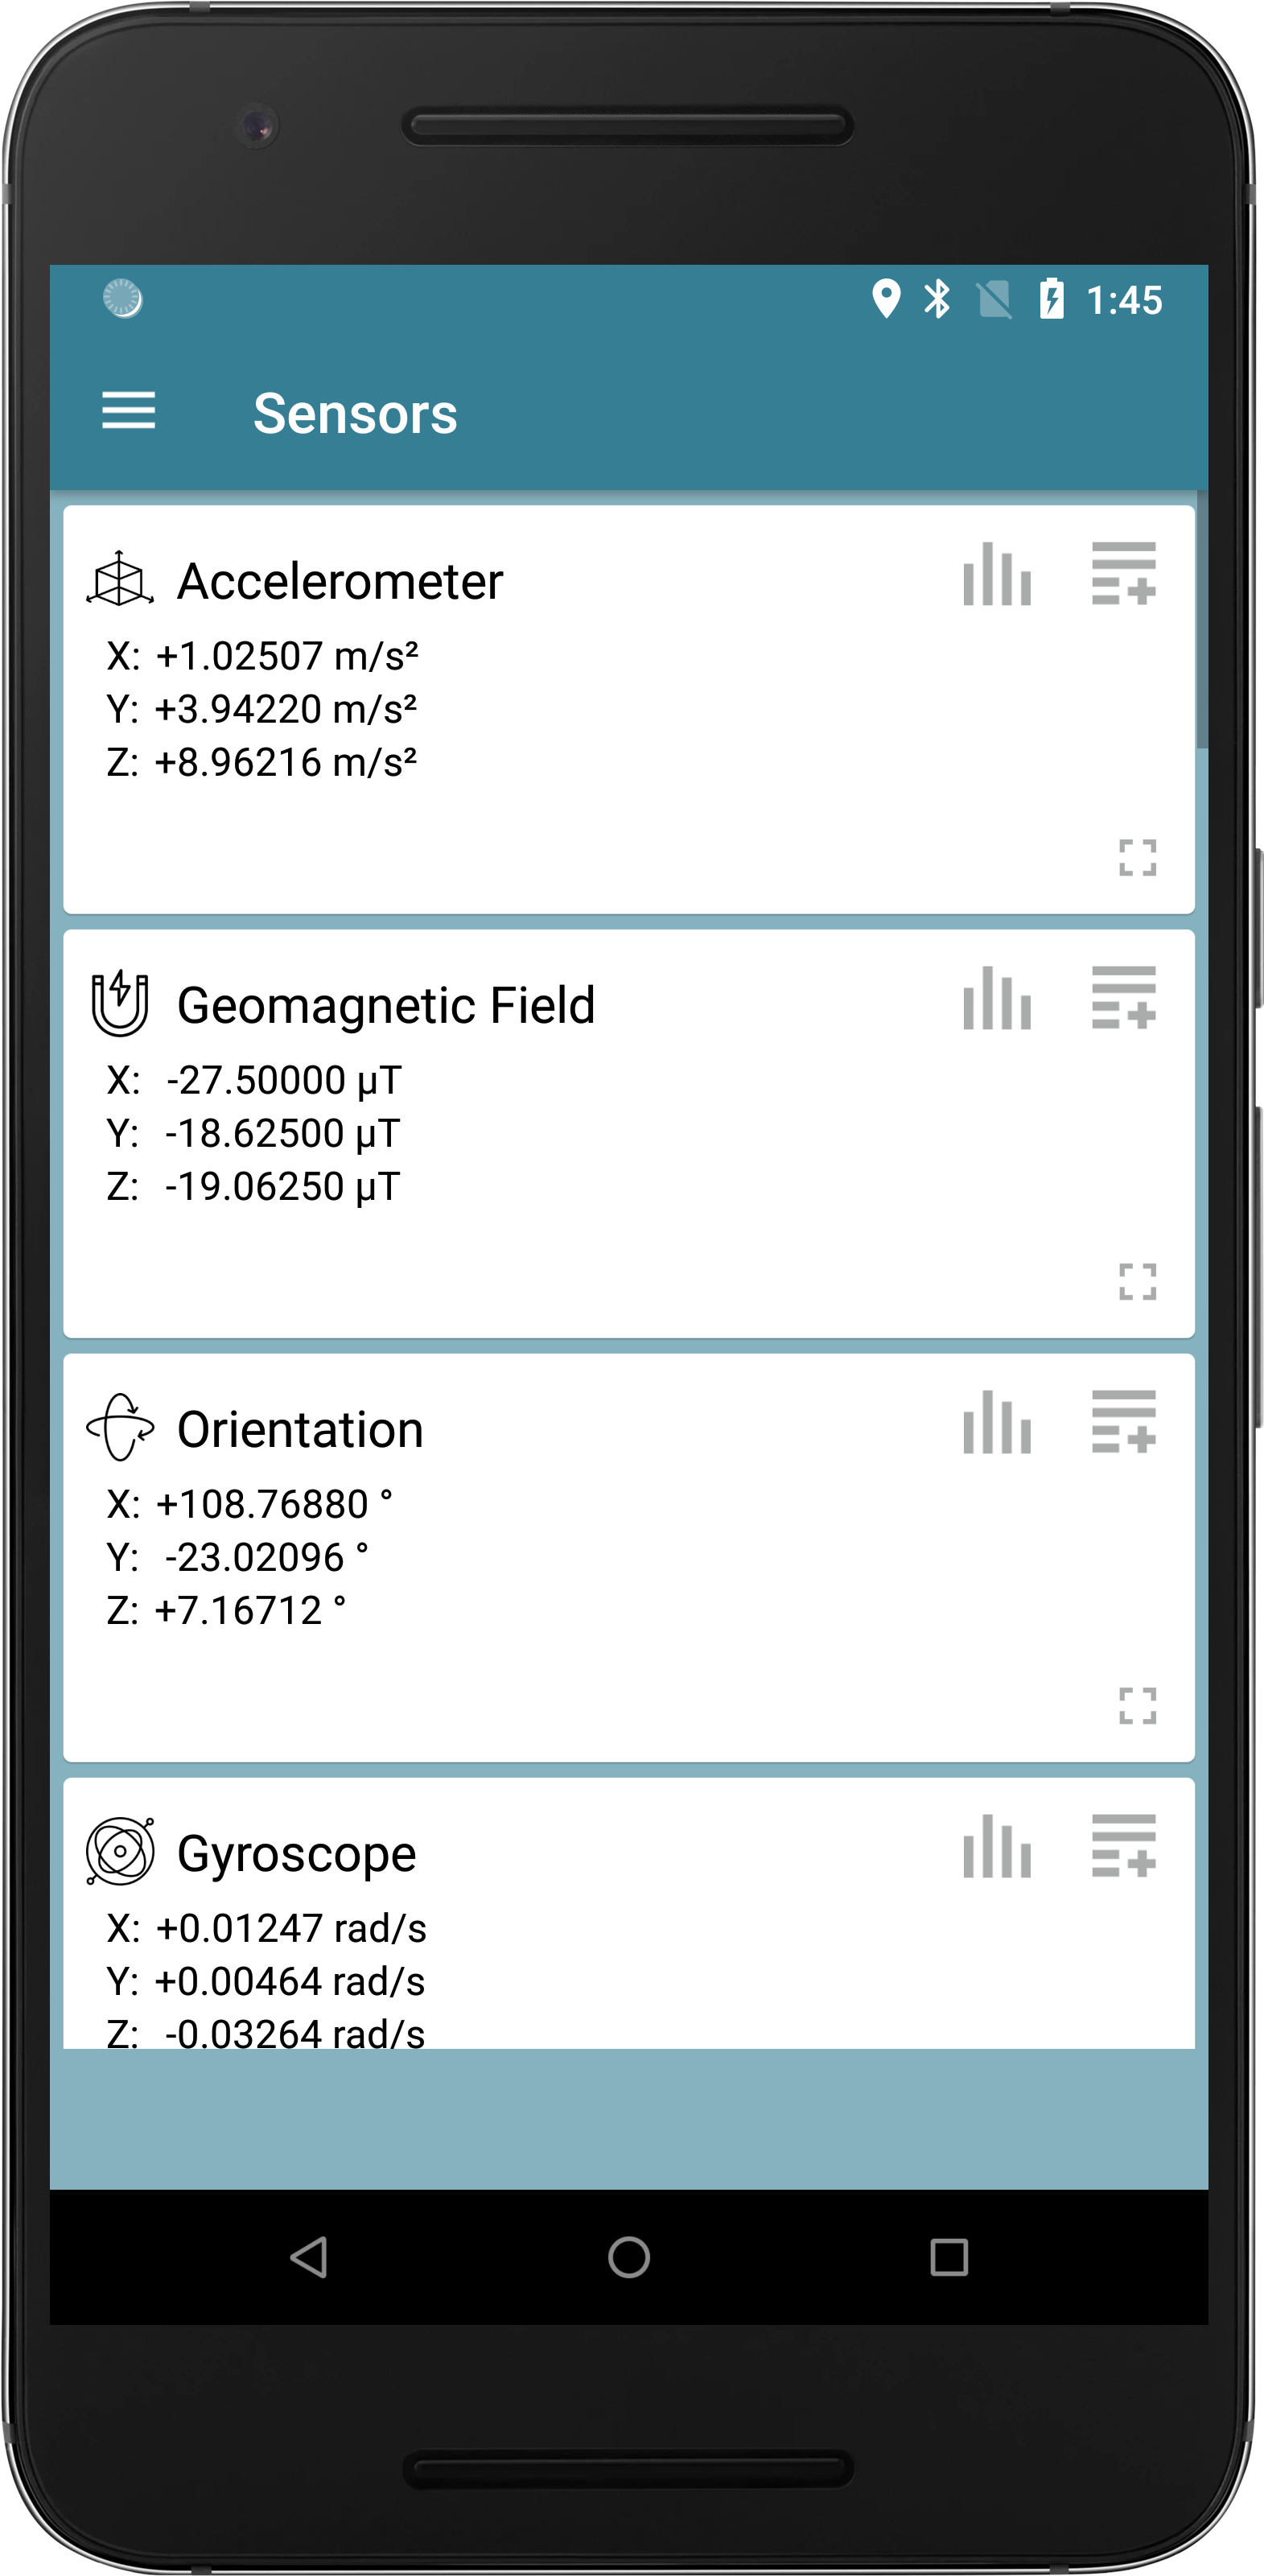
\includegraphics[width=1.4\textwidth]{sensors1}
		\end{minipage}
		\hspace{.60in}
		\begin{minipage}[t]{0.25\textwidth}
			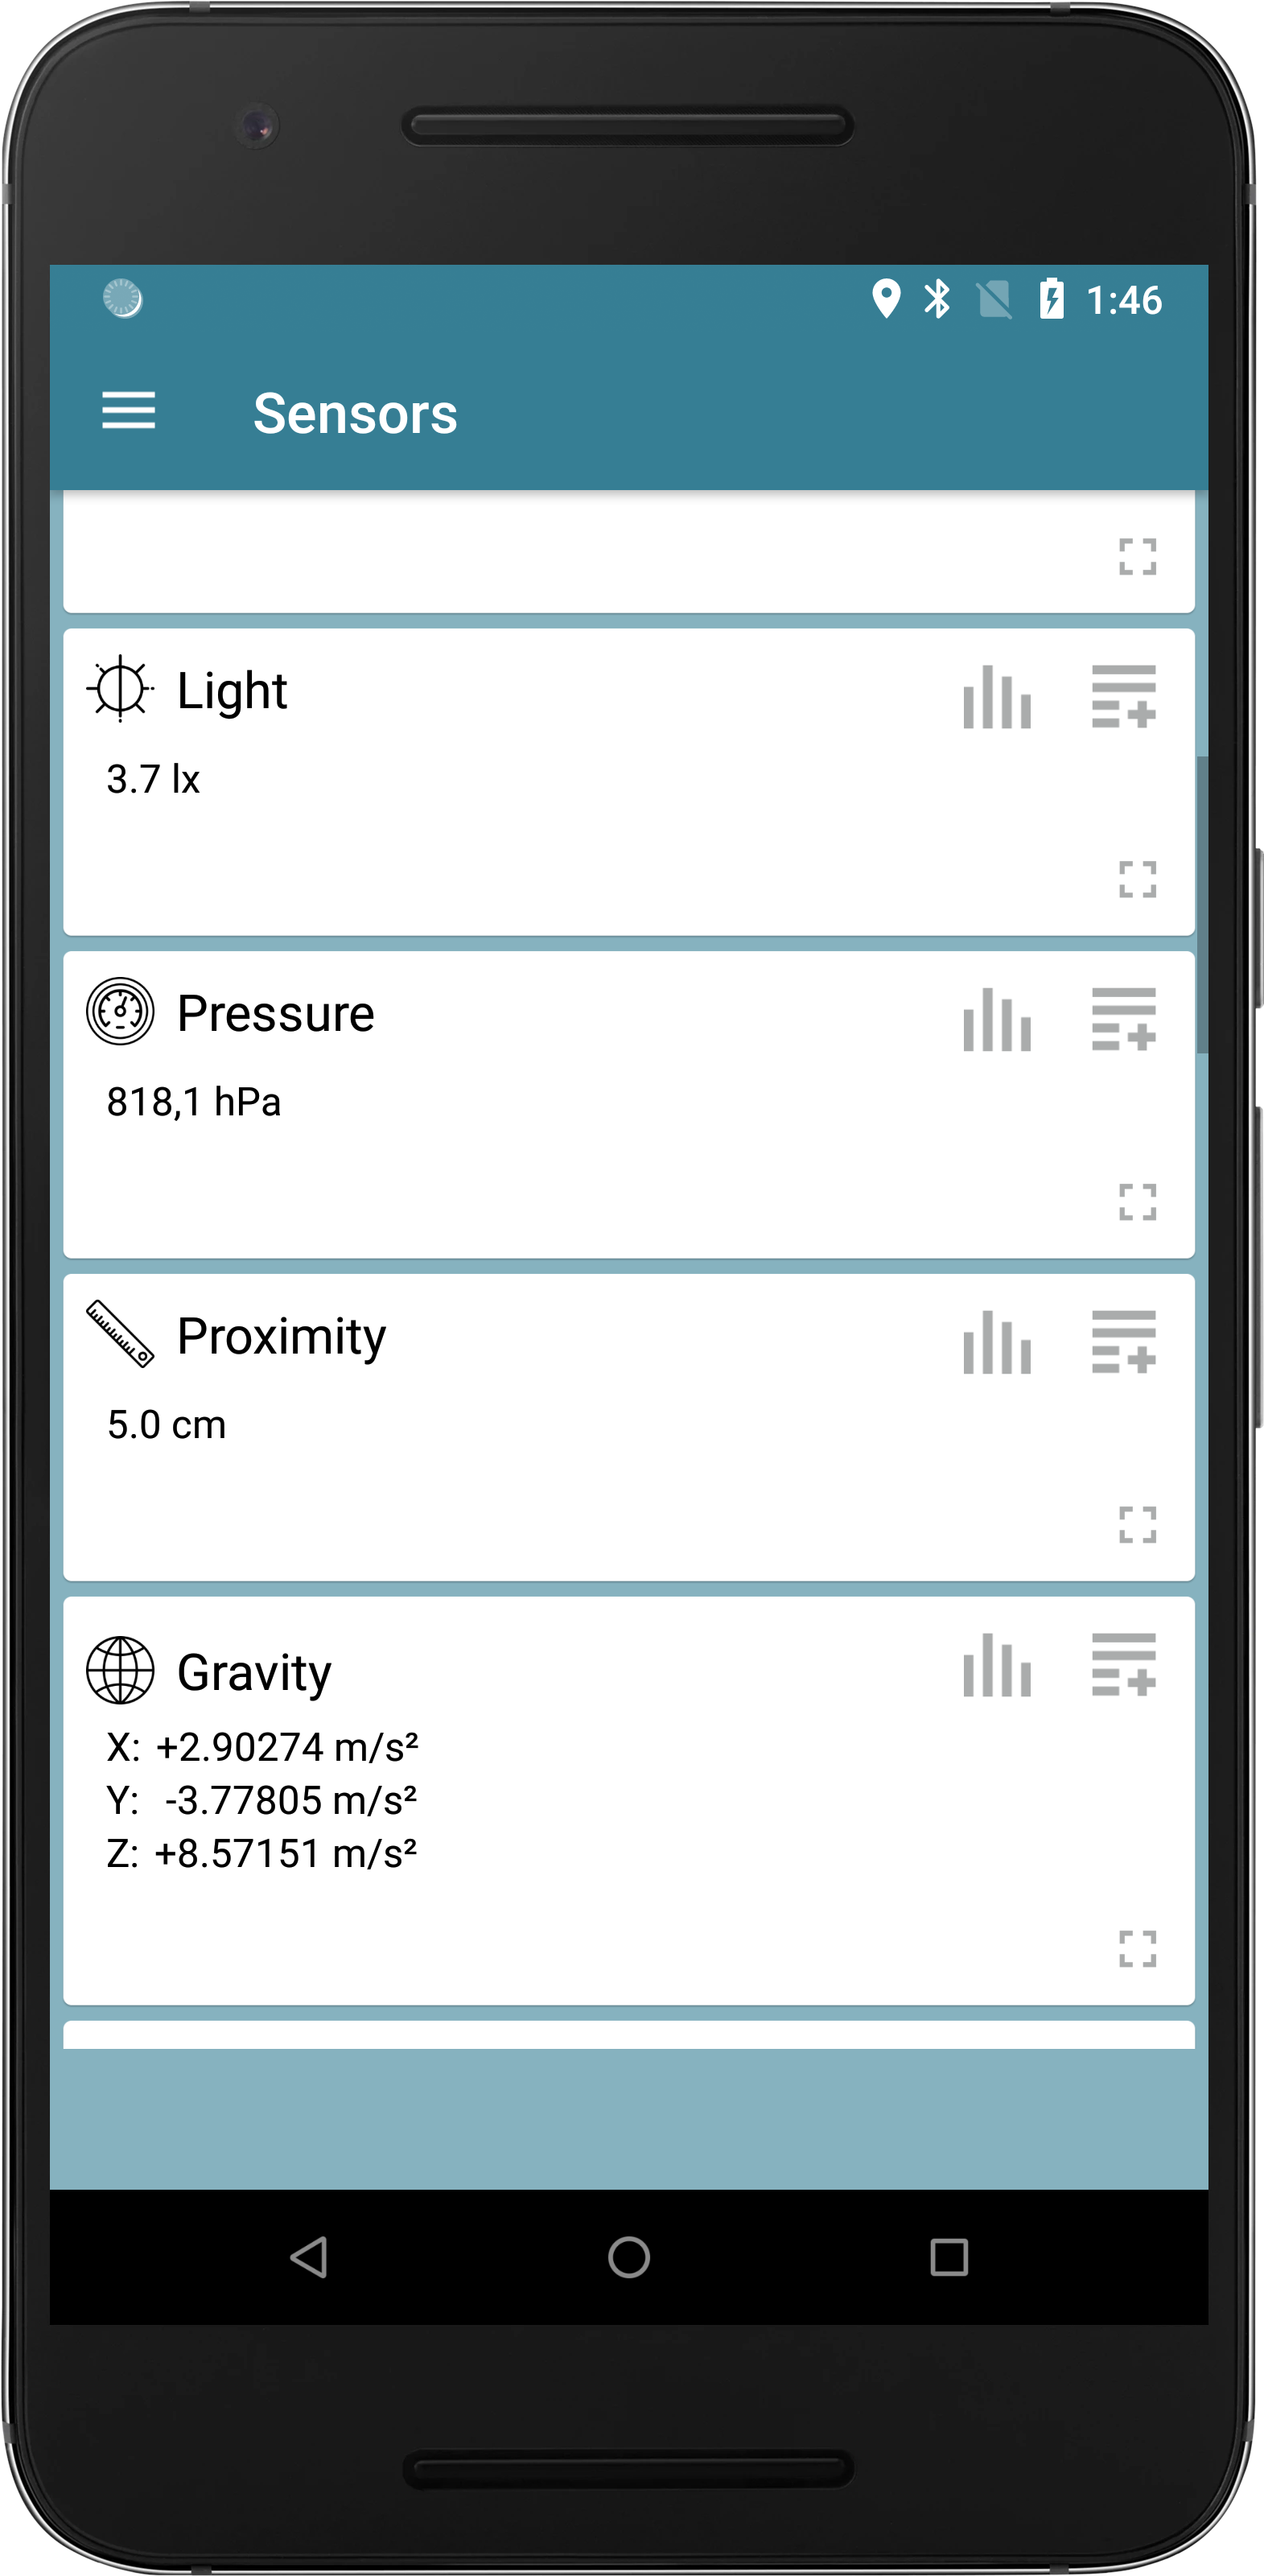
\includegraphics[width=1.4\textwidth]{sensors2}
		\end{minipage}
		\hspace{.60in}
		\begin{minipage}[t]{0.25\textwidth}
			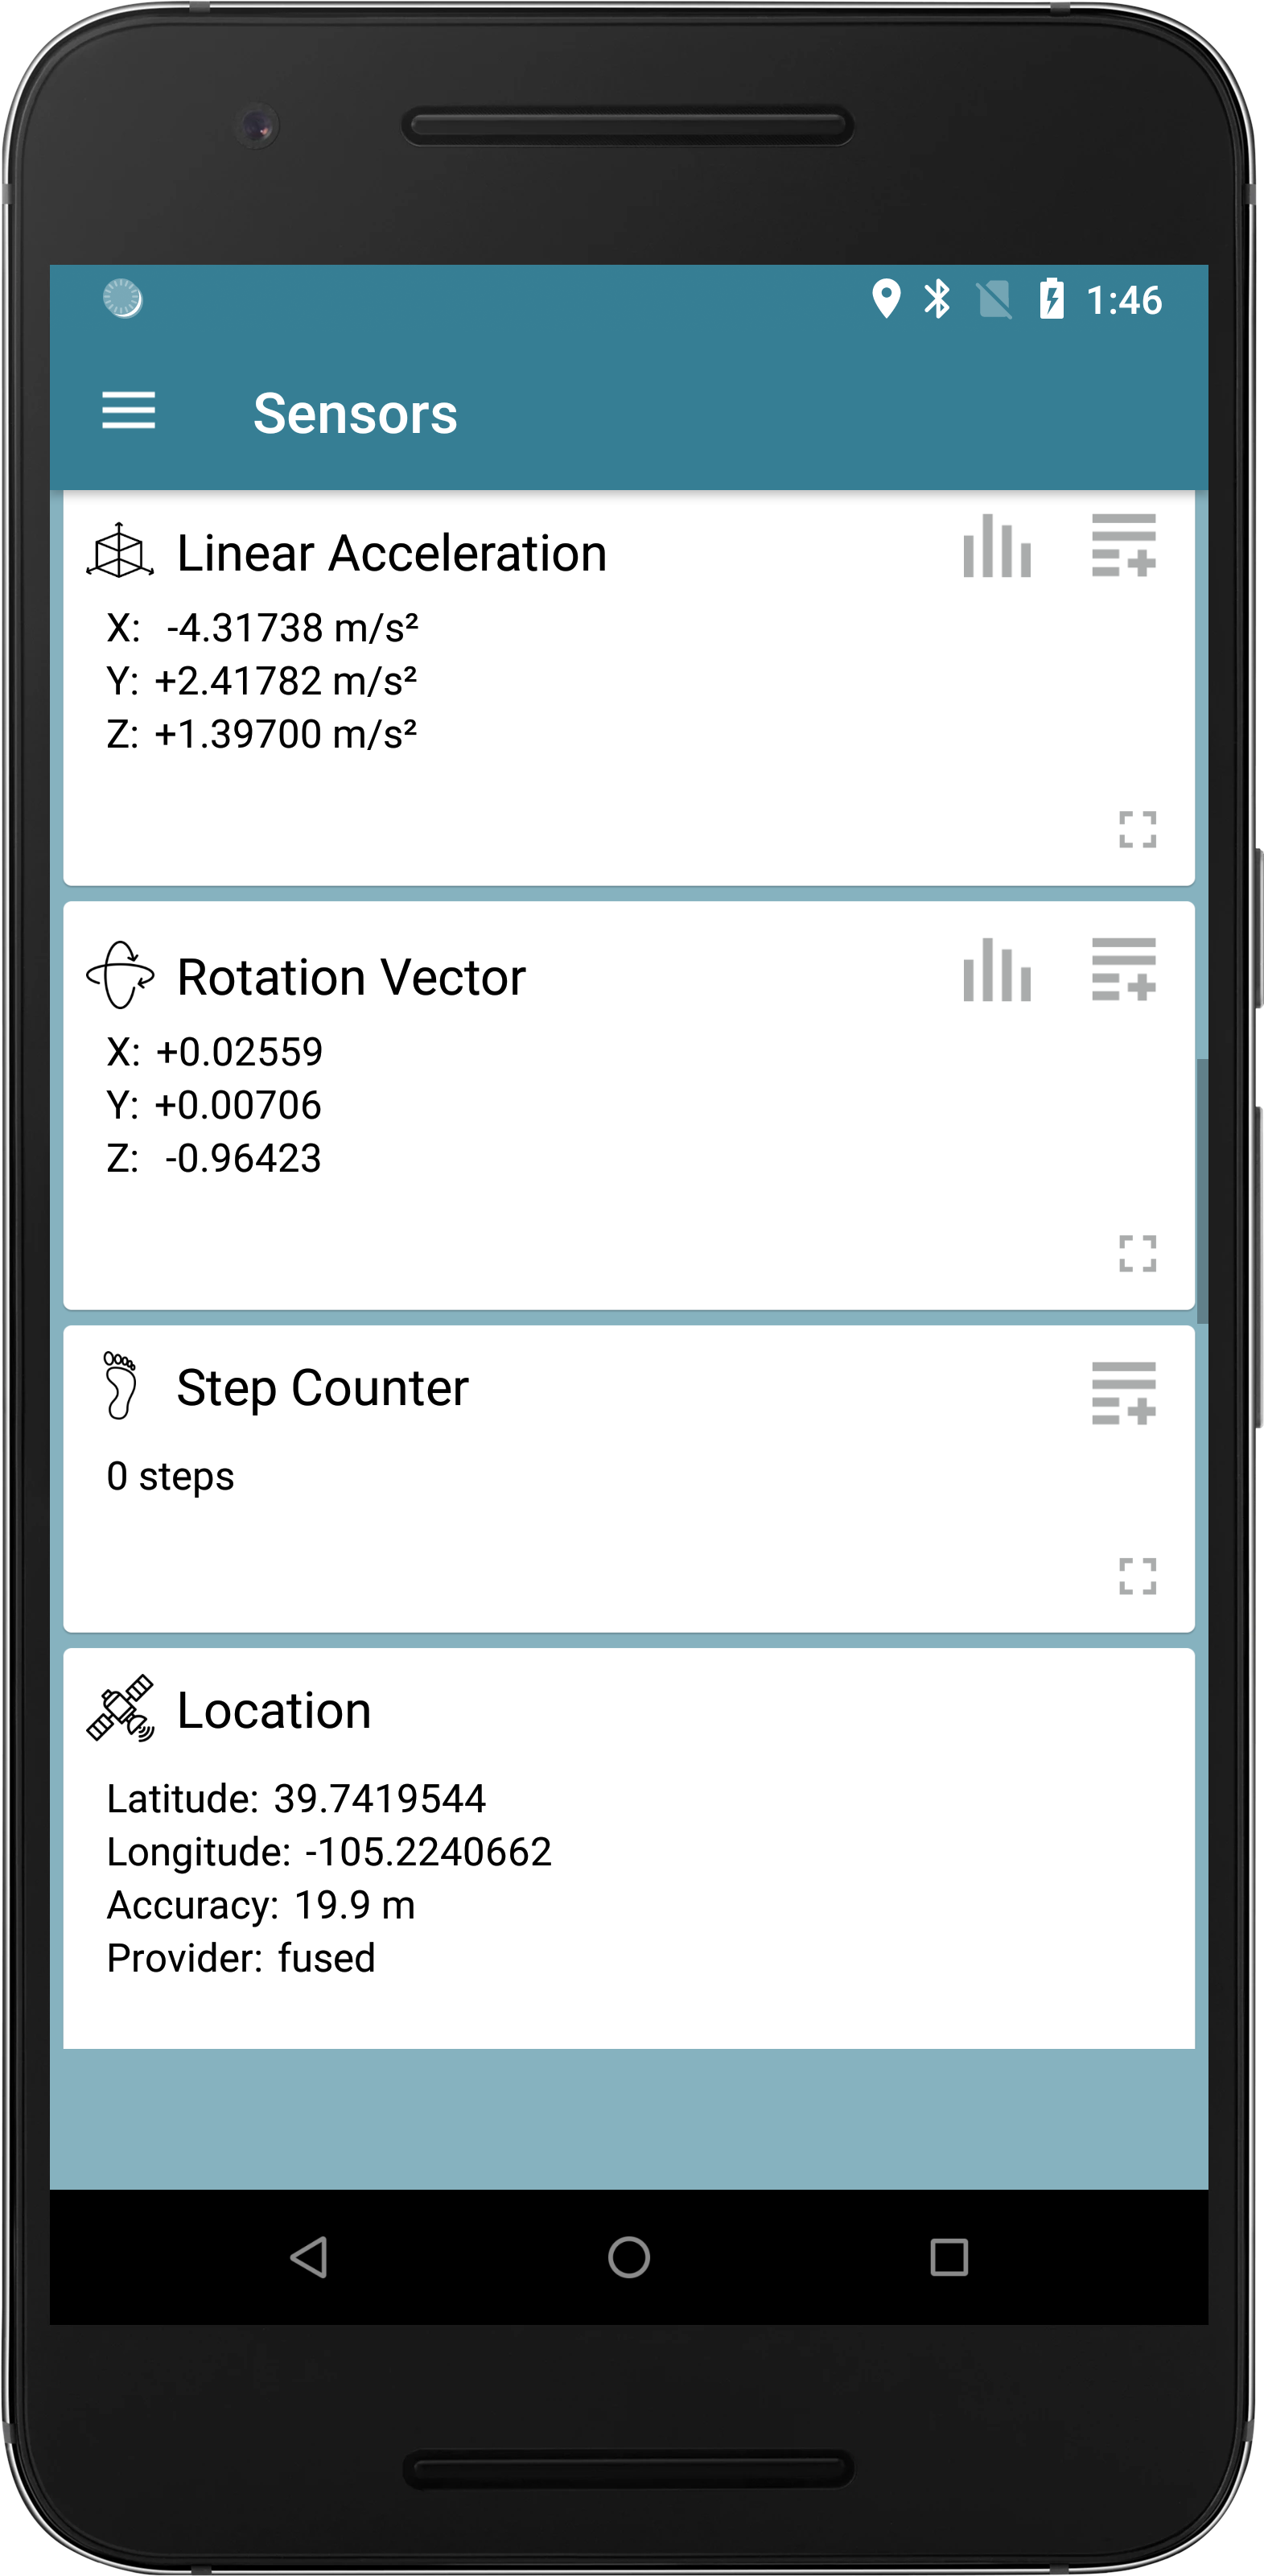
\includegraphics[width=1.4\textwidth]{sensors3}
		\end{minipage}  
		\hspace{.60in}
		\begin{minipage}[t]{0.25\textwidth}
			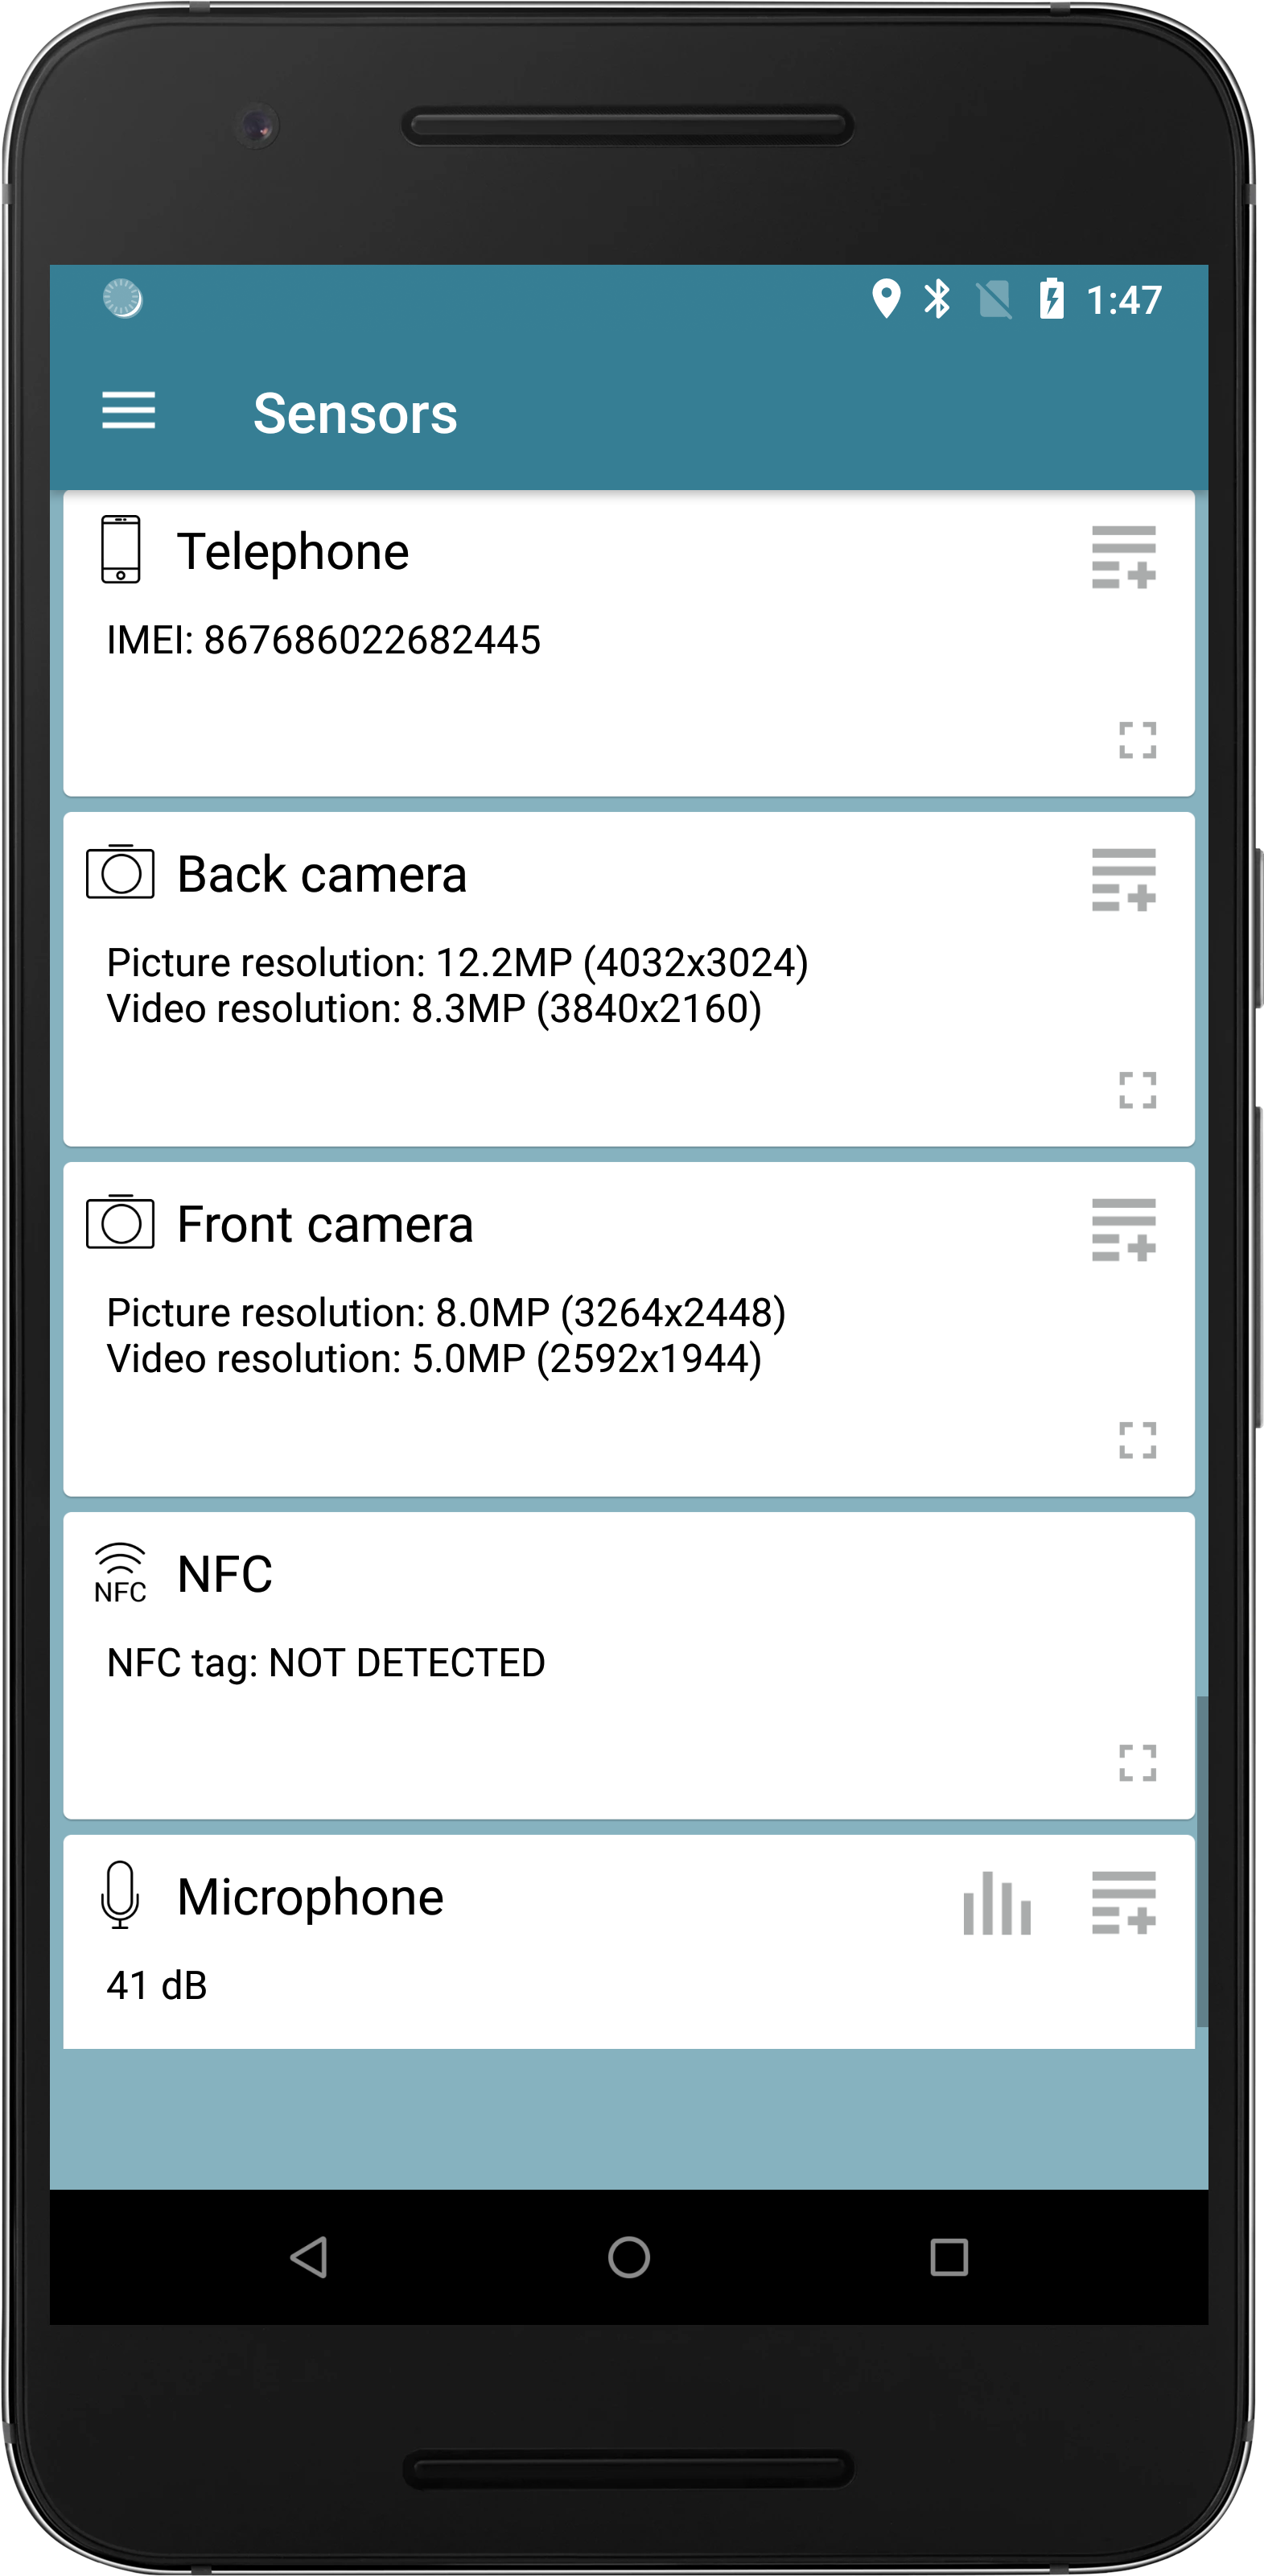
\includegraphics[width=1.4\textwidth]{sensors4}
		\end{minipage}  
		\caption{Real Readings of 18 Sensors on a Google Nexus 6P Device.}
		\label{fig:sensors}
	\end{figure*}
\end{landscape}

%TODO our approach
